%!TEX root = mainfile.tex
\subsection{Spectroscopy} % (fold)
\label{sec:spectroscopy}
(John)

	The spectrum of a typical high redshift galaxy can be seen in Figure~\ref{fig:high_redshift_galaxy_spectrum}.
	\begin{figure}[htbp]
		\centering
			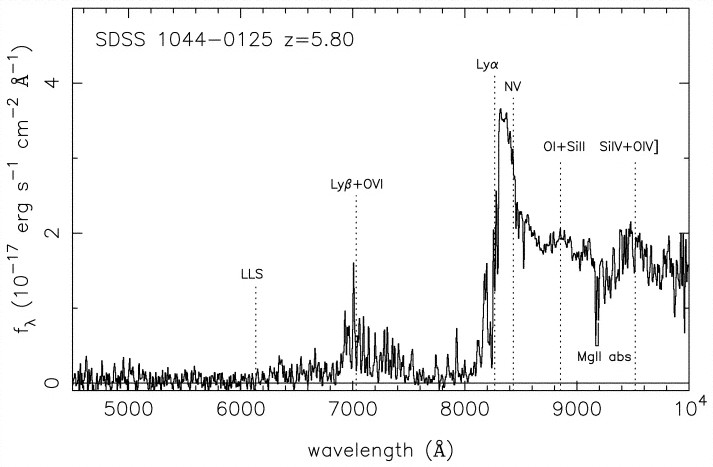
\includegraphics[width=0.7\textwidth]{../Images/high_redshift_galaxy_spec.jpg}
		\caption{\label{fig:high_redshift_galaxy_spectrum} The spectrum of a typical high redshift galaxy}
	\end{figure}

	The distinct drop in emission is due to the presence of neutral hydrogen around the galaxies, known as the Gunn-Peterson trough, therefore the galaxies were formed before the start of reionization. This is discussed in detail in Section~\ref{sec:the_gunn_peterson_effect}. However this particular feature in the spectra is of great importance here. The wavelength at which this drop occurs corresponds to the amount of energy required for an electron to transition between the first two energy levels in neutral hydrogen. This is known as the Lyman-$\alpha$ transition line and has a rest frame wavelength here on earth of \SI{1216}{\angstrom}\cite{LymanAlphaForest}\cite{TransofAtomicH}. However, the actual wavelength that this drop occurs in the spectrum of the galaxy being studied will be much longer. In Figure~\ref{fig:high_redshift_galaxy_spectrum}, it is closer to \SI{8000}{\angstrom}.This is due to the fact that the light is redshifted effectively stretching the wavelength. Indeed, the observed wavelength of the Lyman-$\alpha$ transition line will be in the infrared range. If this wavelength can be measured precisely then the redshift of the galaxy can be calculated\cite{EvidenceRion}. This is done using the relation in equation~(\ref{eq:dropout_wavelength}). Hence, spectroscopy can be used to confirm the high-redshift galaxy candidates that are identified via photometry. In essence it is high resolution photometry.

	An astronomical spectrograph splits or disperses light from a source into its constituent wavelengths. Therefore it has to have some means of dispersing the light. The simplest way this can be achieved is via a prism. This exploits the fact that different wavelengths are diffracted by different amounts. However, they are rarely used by themselves in astronomical spectroscopy due to their inefficiency. Only about 10\% of the light incident upon them actually gets dispersed. Moreover, the dispersion is nonlinear causing some light to be dispersed more than others. Therefore, the universal dispersing medium used in astronomical spectroscopy is the diffraction grating. A diffraction grating consists of a large number of equidistant parallel lines ruled onto a transparent glass plate. The incident light cannot travel through the grating, but is instead channelled along the parallel lines. As the light reaches the end of the lines it is diffracted producing a series of wavelets in accordance with Huygens's Principle. These either constructively or destructively interfere producing a series of maxima or minima. Again, different wavelengths of light will be diffracted through different angles. Therefore each maximum (order) can be thought of as the image of the galaxy split into its constituent wavelengths. As a general rule, the first maximum is projected onto the CCD equipment of the telescope and used to calculate the redshift. This is due to the fact it has the highest intensity. Figures~\ref{fig:grating_to_split_light} and~\ref{fig:grating_close_up} below show a schematic of a grating being used to split light
.	\begin{figure}[htbp]
		\begin{minipage}[c]{0.5\linewidth}
			\centering
			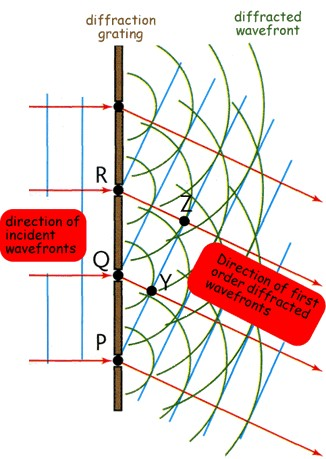
\includegraphics[width=0.7\textwidth]{../Images/grating_to_split_light.jpg}
			\caption{\label{fig:grating_to_split_light} Schematic of a grating}
		\end{minipage}
		\begin{minipage}[c]{0.5\linewidth}
			\centering
			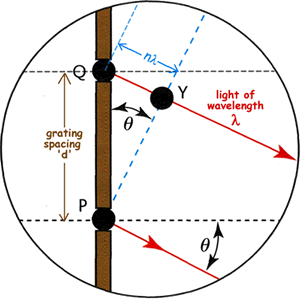
\includegraphics[width=0.7\textwidth]{../Images/grating_close_up.png}
			\caption{\label{fig:grating_close_up} Path difference due to diffraction}
		\end{minipage}
	\end{figure}

	Angles at which the orders occur can be found using the grating equation\cite{DiffGrating},
	\begin{align}
		n\lambda &= d(\sin\theta + \sin\phi)
	\end{align}
	where $\phi$ is the angle of incidence between the light and the grating, $\theta$ is the angle of dispersion and $d$ is the grating spacing. The value of $n\lambda$ is an integer number of wavelengths of the incident light.

	Before light reaches either a prism or diffraction grating it is often sent through a fixed slit. This is a mask with a narrow rectangular aperture that is placed in the focal plane of the telescope. The slit has two main functions. First and foremost it isolates the portion of the sky of interest so that only light that falls on the slit may enter the spectrograph. This is important as it means the spectra from different parts of a galaxy cannot enter the spectrograph, overlap and thus contaminate each other. Second, the slit provides a stable spectral resolution; without the slit the spectral resolution would be defined by the width of the galaxy or star. However, this varies with time so the spectral line width would vary with time. This would make detailed analysis of the spectrum almost impossible. If on the other hand a slit is used, the spectrum becomes an infinite number of images of the slit, and not the galaxy or star etc. As the slit width is constant, the spectral resolution remains stable\cite{SpectoG}.

	In between the slit and dispersion medium usually sits a collimator. The light from the slit diverges and if left would hit the grating or prism at differing angles of incidence making the resulting spectrum useless. Therefore a collimator is used to turn the diverging light back to parallel. Figure~\ref{fig:nirspec_jwst} below shows the set-up for NIRspec on the JWST.
	\begin{figure}[htbp]
		\centering
			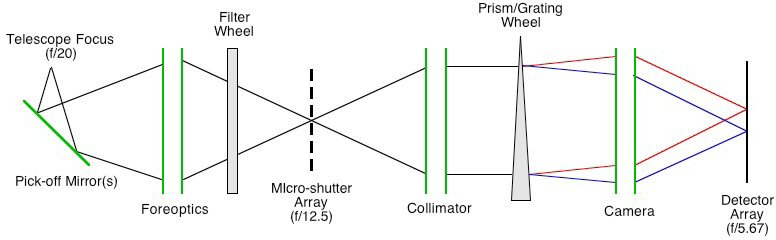
\includegraphics[width=0.8\textwidth]{../Images/nirspec_jwst.jpeg}
		\caption{\label{fig:nirspec_jwst} Schematic of JWST's NIRspec}
	\end{figure}

	Grisms are a combination of both diffraction gratings and prisms. In some cases they enable spectroscopy and photometry to be undertaken simultaneously. This is achieved by using the dispersed and undispersed light that they produce. This means that exposure times can be shortened when viewing and confirming high redshift galaxy candidates.
% section spectroscopy (end)

